%\documentclass[wcp,gray]{jmlr} % test grayscale version
\documentclass[wcp]{jmlr}

% The following packages will be automatically loaded:
% amsmath, amssymb, natbib, graphicx, url, algorithm2e

%\usepackage{rotating}% for sideways figures and tables
\usepackage{longtable}% for long tables

% The booktabs package is used by this sample document
% (it provides \toprule, \midrule and \bottomrule).
% Remove the next line if you don't require it.
\usepackage{booktabs}
% The siunitx package is used by this sample document
% to align numbers in a column by their decimal point.
% Remove the next line if you don't require it.
%\usepackage[load-configurations=version-1]{siunitx} % newer version
\usepackage{siunitx}

% The following command is just for this sample document:
%\newcommand{\cs}[1]{\texttt{\char`\\#1}}

\jmlrvolume{vol}
\jmlryear{2012}
\jmlrworkshop{Workshop Title}

\title[RRTPI]{Policy Iteration on Continuous Domains using Rapidly-exploring Random Trees}

 % Use \Name{Author Name} to specify the name.
 % If the surname contains spaces, enclose the surname
 % in braces, e.g. \Name{John {Smith Jones}} similarly
 % if the name has a "von" part, e.g \Name{Jane {de Winter}}.
 % If the first letter in the forenames is a diacritic
 % enclose the diacritic in braces, e.g. \Name{{\'E}louise Smith}

 % Two authors with the same address
%  \author{\Name{Author Name1} \Email{abc@sample.com}\and
%   \Name{Author Name2} \Email{xyz@sample.com}\\
%   \addr Address}

 % Three or more authors with the same address:
 % \author{\Name{Author Name1} \Email{an1@sample.com}\\
 %  \Name{Author Name2} \Email{an2@sample.com}\\
 %  \Name{Author Name3} \Email{an3@sample.com}\\
 %  \Name{Author Name4} \Email{an4@sample.com}\\
 %  \Name{Author Name5} \Email{an5@sample.com}\\
 %  \Name{Author Name6} \Email{an6@sample.com}\\
 %  \Name{Author Name7} \Email{an7@sample.com}\\
 %  \Name{Author Name8} \Email{an8@sample.com}\\
 %  \Name{Author Name9} \Email{an9@sample.com}\\
 %  \Name{Author Name10} \Email{an10@sample.com}\\
 %  \Name{Author Name11} \Email{an11@sample.com}\\
 %  \Name{Author Name12} \Email{an12@sample.com}\\
 %  \Name{Author Name13} \Email{an13@sample.com}\\
 %  \Name{Author Name14} \Email{an14@sample.com}\\
 %  \addr Address}


 % Authors with different addresses:
 % \author{\Name{Author Name1} \Email{abc@sample.com}\\
 % \addr Address 1
 % \AND
 % \Name{Author Name2} \Email{xyz@sample.com}\\
 % \addr Address 2
 %}

%\editor{Editor's name}
% \editors{List of editors' names} 

\begin{document}

\maketitle

\begin{abstract}
Reinforcement Learning on continuous states and continuous actions is a challenging task. Several techniques in the literature use function approximations and data from sample trajectories to solve it. They however, do not mention how to generate these samples. We present a method of generating samples using Rapidly-exploring Random Trees(RRTs). We also introduce a new policy iteration based algorithm RRTPI that iteratively learns an optimal policy by using these samples as an approximate representation of the policy and improving them using a novel approach. The algorithm is free from learning rates and other exploration parameters. We also present some ideas that could lead to proving the samples generated through RRTs maybe fast-mixing. The sample efficiency of our algorithm is shown empirically by evaluating it in a simple domain. 
\end{abstract}
\begin{keywords}
Approximate policy iteration, continuous state action, RRTs, model based
\end{keywords}

\section{Introduction}
Reinforcement Learning(RL) deals with learning optimal control strategies through interactions with the world. One of the major hindrances in extending existing RL techniques to real world scenarios, is their inability to deal with continuous valued variables. Techniques such as discretization exist but a better way to handle this is to use function approximators in place of lookup tables in the original discrete space algorithms. Least Squares Policy Iteration(LSPI) introduced in \citep{lspi} is an offline method that uses a set of experiences and linear function approximators. Although LSPI is a fundamentally sound algorithm, the question of how exactly the experiences should be generated exists. In \citep{rmaxlspi} the authors try to address this problem of online exploration in large domains by combining LSPI with R-MAX, a technique that does efficient exploration in discrete domains. Several implementation issues arise in translating this to continuous domains, such as tuning exploration parameters and generalizing state visitation counters. \citep{antosml} also describe a policy iteration based algorithm that learns from sample experiences and in their analysis, they state the need for the sample set to be sufficiently ``rich". Ng and Jordan in \citep{pegasus} make use of a model of the domain to make the problem tractable.\\
 In this paper, we propose a policy iteration based algorithm - RRTPI that combines ideas from the domain of continuous planning to clearly provide a method to generate sufficiently representative samples and ensure exploration. Our work makes use of Rapidly-exploring Random Trees(RRTs), a widely popular continuous domain planning technique introduced by Lavalle in \citep{rrt}. RRTs have several attractive properties that we exploit - they are parameter free and have provable exploration properties. 
\sectionref{sec:prelims} introduces Markov Decision Processes and the policy iteration algorithm. The next \sectionref{sec:rrt} gives a brief description about RRTs. The details of the proposed algorithm and discussion are presented in \sectionref{sec:rrtpi}. Some basic experimental results are discussed in \sectionref{sec:experiment}.

\section{Preliminaries}
\label{sec:prelims}
A Markovian Decision Process(MDP) is described as $\left\langle S,A,P,R\right\rangle$, where $S\in \mathbb{R}^n$ is the domain of states and $A\in \mathbb{R}^m$ is the domain of actions. $P$ is the state transition probability. $R$ is a real valued reward function. The aim of the \textit{RL agent} is to maximize the discounted cumulative reward obtained.
A deterministic policy $\pi$ is a mapping from the state space $S$ to the action space $A$. $V^\pi(s)$ is the state value function and is equal to the expected long term rewards, by following $\pi$ at $s$. Similarly, $Q^\pi(s,a)$ is the state-action value function. The value function might be expressed as,
\begin{equation}
\label{eq:Vbell}
\forall s \in S,\;\; V^\pi(s) = R(s) + \gamma \sum_{s'}P^{ss'}_{\pi(s)}V^\pi(s')
\end{equation}
where $s'$ is the state transitioned to and $\gamma \in \left(0,1\right)$ is the discount factor. A policy $\pi^*$ is optimal if $ \forall s,\pi\;\; V^{\pi^*}(s)\geq V^\pi(s) $ The optimal value function can be calculated by replacing the expectation in \equationref{eq:Vbell} with $\max$.

\subsection*{Approximate Policy Iteration}
 If the state space is discrete, we can use techniques such as policy iteration or value iteration to solve \equationref{eq:Vbell}. In most problems however, the probability distribution $P^{ss'}_a$ is unknown or hard to compute. In which case, the agent has to learn only through interactions with the world. This interaction experience is usually represented as a set of tuples of the form $(s,a,s',r)$ corresponding to the current state, action taken, the next state and the reward obtained respectively. In most cases a \textit{generative model} as in \citep{kearns99} is available that allows the agent to generate such tuples from arbitrary states. \\
In the domain of continuous states and continuous actions, we have to use approximate representation using function approximators. Using such approximate representations in the policy evaluation and improvement steps is referred to as \textit{approximate policy iteration} \citep{neurodp}. This represents a popular section of the methods such as those presented in \citep{lspi},\citep{rmaxlspi} and \citep{antosml}. The algorithm we present also fits into the approximate policy framework.\\
There are several methods that use  linear function approximators of the form $V(s) = \vec{\phi(s)}^T\vec{w} $, where $\phi$ is a basis function. Least Squares Temporal Difference(LSTD $ (\lambda ) $ ) discussed in \citep{lstd} assumes such a form and uses weighted linear regression to estimate the state value function $V$. \citep{antosml} also use a linear model to approximate the state-action value function $Q$. Another popular technique is Fitted Q-Iteration The algorithm calculates a set of regressors each corresponding to the $k^th-step$ value function estimate. FQI may be summarized as: \\Given a set interaction experiences $\mathcal{D}$  that contains tuples of the form $(s,a,s',r)$, iteratively calculate \[Q_{k+1} = Regress\left( \left[ \phi(s_i,a_i), r_i+\gamma \max_{b\in A}Q_k(s_i',b) \right]_{1 \leq i \leq \vert \mathcal{D}\vert } \right) \] 
The $Regress$ function is generic and any technique such as neural nets, linear regression and regression trees might be used. To evaluate a given policy $\pi$ we may use a similar approach:\\
Given a set interaction experiences $\mathcal{D}$ , iteratively calculate

\begin{equation}\label{eq:fpe}
V^\pi _{k+1} = Regress\left( \left[ \phi(s_i), r+\gamma P^{s_is_i'}_{\pi(s_i)}V^\pi _k(s_i') \right]_{1 \leq i \leq \vert \mathcal{D}\vert} \right)
\end{equation} 

We will refer to this as Fitted Policy Evaluation(FPE). Several works based on approximate policy iteration such as \citep{rmaxlspi} and \citep{lspi}, prefer to evaluate $Q(s,a)$ as opposed $V(s)$ in the policy evaluation step. The main reason being it simplifies the policy improvement step. In our work we choose working with $V$ function for the following reasons:

\begin{itemize}
	\item In RL problems with continuous states and actions, the $Q$ value for different actions at the same state will not differ as much as the $Q$ value at different states given that the state-action space is smooth. As pointed out by Baird in \citep{bairdadvantage} , as the time step between actions decreases, the policy implied by the $Q$ values becomes more sensitive to bias in the function approximation.
	\item We introduce a method by which we can use the $V$ function to improve the policy
	\item Implementing the $\max$ operator for continuous action spaces is difficult.
\end{itemize}

When in theory any algorithm that approximates the $V$ function given a set of experiences suffices, empirically FPE was found to be the most stable. In our work we use FPE to evaluate $V$ in the policy evaluation step. The reader should note that the actual $P^{ss'}_{\pi(s)}$ is not needed although it appears in the equation. In the next section we outline a technique of generating the sample set $ \mathcal{D}$ using RRTs.

\section{Rapidly-exploring Random Trees}
\label{sec:rrt}
\begin{figure}[htb]
% Caption and label go in the first argument and the figure contents
% go in the second argument
\centering
\label{fig:rrt}
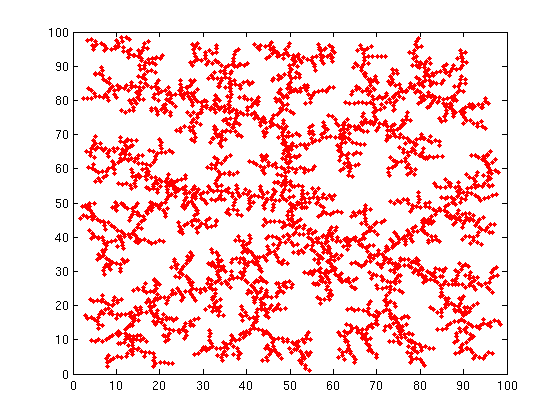
\includegraphics[scale=0.4]{rrt.png}
\caption{RRT with 3000 nodes grown in $(0,100)^2$ starting from (50,50)}
\end{figure}

The basic RRT construction is outlined in \algorithmref{alg:basicrrt}. The algorithm is straightforward and elegant and there are no explicit parameters that must be set. \figureref{fig:rrt} shows a RRT grown in a 2 dimensional space. RRTs have been shown to be \textit{probabilistically complete} by Kuffner and Lavalle in \citep{rrtconnect}. In other words, the probability of reaching any point in space approaches 1 as the size of the tree increases. Hence it can be shown that 
\begin{lemma}\label{thm:rrt1}
In a RRT, the probability of choosing a node to be extended is proportional to the size of its Voronoi region.
\end{lemma}


\begin{algorithm2e}
\caption{ConstructRRT}
\label{alg:basicrrt}
\dontprintsemicolon
\Repeat{termination}{Uniformly sample a state $s$\;
Calculate closest point in tree to $s$\;
Extend the tree from the closest point towards $s$ }
\end{algorithm2e}

The RRT can be biased according to any arbitrary pdf by biasing the sampling in step 1 of the algorithm accordingly. 

\section{RRTPI}
\label{sec:rrtpi}
The proposed algorithm uses a technique based on RRTs to generate samples trajectories in state space of the given MDP. By using these samples, the value function is calculated using Fitted Policy Evaluation as described in \equationref{eq:fpe}. The key step in the RRTPI algorithm is using the value function $V$ to bias the generation of trajectories in the next iteration, thus completing the loop of policy iteration.
We first introduce Rapidly-exploring Random Sample Trees(RRSTs) that generate sample experiences using the RRT framework. The following assumptions are made:
\begin{enumerate}
\item A generative model $\mathcal{M}$ that allows us to sample the reward function given a state transition.
\item An \textit{approximate local controller} that can move from a given state to any state in its neighborhood. Note that this controller may not always move to the intended target state due to stochasticity in the state transitions.
\end{enumerate}

These assumptions seem reasonable in continuous state and action space MDPs such as problems in the domain of robotics. Similar assumptions are made in \citep{partigame} and \citep{pegasus}. \algorithmref{alg:rrst} constructs a RRST takes as input a PDF $ g $  defined over the state space $S$ of the MDP and a starting state and outputs a sample tree that has $N$ nodes. The set of experience samples $\mathcal{D}$ is also populated. The function \textit{ExtendTowards} invokes the local planner at state $s_{near}$ to move it towards some $s'$ in the direction of the random sample $s_{sample}$. The resulting RRST is biased according to $g$.\\
Each leaf of the RRST can be traced back along a trajectory of states to the starting state. Thus the RRST can be thought of as compact representation of several trajectories. Thus the RRST is also an approximate representation of the policy in the RRTPI algorithm.\\

\begin{algorithm2e}
\caption{ConstructRRST$(g)$}
\label{alg:rrst}
\dontprintsemicolon
Initialize tree $\mathcal{T}$ with node $s_{init}$\;
Initialize set $\mathcal{D} \leftarrow \emptyset$\;
\While{size of $\mathcal{T} \leq N$}{
$s_{sample} \sim g(s)$\;
$s_{near} \leftarrow NearestNode(s_{sample},\mathcal{T})$\;
$s' \leftarrow ExtendTowards(s_{near},s_{sample})$\;
\If{ExtendSuccessful}{
$r\sim \mathcal{M}(s,s')$\;
Add  Edge $(s,s')$ to $\mathcal{T}$\;
$D \leftarrow D \cup \left(s_{near},s',r \right)$\;
}
}
\end{algorithm2e}
 The RRTPI algorithm is shown in  \algorithmref{alg:rrtpi}. We now present a method of sampling from a probability distribution $g$ where  $g(x) \propto V(x),\;\;x\in S$. We use a particle set approximation to do this. First we uniformly sample $M$ points from the state space. Let these be the set $\{x_m\}$. We initialize weights correspond to each samples as $w_m \leftarrow V(x_m) $. The next step is to make all weights positive and sum to 1 by subtracting the minimum and then \textit{normalizing} them. We then re-sample the particle set $\{x_m,w_m\}_{1\leq m \leq M}$ according to its weight $w_m$. In other words, we choose with replacement $M$ particles from the set such that, the probability of choosing a particle $x_i$ is proportional to the weight $w_i$. It can now be proved that sampling uniformly from this new sample set is approximately equivalent to sampling a point according to the pdf $g$. The error in this approximation approaches 0 as the number of samples $M \rightarrow \infty$. This is step 2 in the RRTPI algorithm. It can be shown that steps 3 and 4 correspond to approximate policy improvement and approximate policy evaluation respectively.

\begin{algorithm2e}
\caption{RRTPI}
\label{alg:rrtpi}
\dontprintsemicolon
\nl Initialize value function uniformly $V\leftarrow \vec{0}$\;
\Repeat{convergence is achieved}{
\nl Construct pdf $g$ from function $V$\;
\nl \textbf{Policy Improvement:}$\;(\mathcal{T,D}) \leftarrow ConstructRRST(g) $\;
\nl \textbf{Policy Evaluation$\;\;\;\;\;$:} $\;V\leftarrow FPE(\mathcal{D})$\;
}
\end{algorithm2e}

\subsection*{Fast Mixing Properties}
Some of the theoretical guarantees of RRTs can be proved through Random Geometric Graph(RGG) theory. The authors of \citep{karaman}, present a variation of RRTs that is asymptotically optimal in the continuous planning sense. The connections between RRTs and RGGs have been introduced in the same work.\\
A random $r$-disc graph $G(n,r)$ is a graph with n vertices in some space. An edge exists between any two vertices if the distance between them is less than r. Of particular interest is connectivity of such graphs. It can be shown that connectivity is a phase transition phenomenon depending on a critical radius $r_{con}$. In particular $Pr(G(n,r)\;\;is\;\;connected)=1,\;\text{if}\;r>(log(n)/n\zeta_d)^{1/d}$ in the limit $n\rightarrow \infty $, where d is the dimension of the points and $\zeta_d$ is volume of the d-dimensional unit ball.
Such critical radii exist in other models of random geometric graphs as well, such as the one that connects the k-nearest neighbors of a node. It can be shown that the radius required for the graph to be rapid mixing $r_{rapid} = \omega(r_{con})$ from \citep{chenavin}.\\
Thus by making some modifications to the basic RRT structure of the sampling procedure(and possibly in the pol. improv. step), essentially connecting to points only within a radius greater than the critical radius as given in the RRT* algorithm of \citep{karaman}, we may be able to prove that the trajectories thus generated are (i)~Fast-mixing (ii)~Have non-zero probability of visiting any given state. These seem to be assumptions needed in proving the sample bounds on the performance of the algorithm.


\subsection*{Discussion}
RRSTs possess  all the exploratory properties of RRTs. The exploration is guaranteed to reach every state in the domain asymptotically. The entire algorithm is free from learning rates and exploration control parameters. The size of the particle set $M$ and the experience sample set $N$ must be set. It is clear that larger these values, better the approximation. Growing RRTs in general is very fast as it can be efficiently implemented using techniques such as k-d trees.\\
It can be shown that the stochasticity in the state transitions does not affect the exploratory properties of the RRST. Suppose the stochasticity caused the tree to be pulled in one particular direction, then according to \lemmaref{thm:rrt1} the probability of extending the tree towards the other directions increases. Thereby ensuring that the bias in the growth of the tree is only due to the pdf used. This enables us to ignore the $P^{ss'}_{\pi(s)}$ in \equationref{eq:fpe} as discussed earlier. This might be an artifact of local controller assumption.\\
The RRST does not represent a single trajectory but several(corresponding to each leaf). By calculating $V$ at the leaf node, the trajectories could be ranked. This could give us a method of discovering equivalent optimal policies or good alternative policies. RRTPI is different from sampling uniformly at random in the space, as it gives samples that can be linked together by the local controller. It is also better than better than building trajectories by randomly sampling a state in the neighborhood of the current state as the space filling properties would not hold in that case. Another advantage of RRTPI is that it gets around the problem of implementing the $max$ operator which is problematic in MDPs with continuous actions and states.\\

\section{Experimental Results}
\label{sec:experiment}
The RRTPI algorithm was tested on a 2-D continuous puddle world. The obstacles and the goal region are terminal states. When one of the leaves reaches these states, the corresponding branch of the tree is not grown further. \figureref{fig:puddle} shows the RRST in the first iteration. Regression trees were used to approximate the value function visualized in \figureref{fig:vfunc}.\\
 We empirically show the sample efficiency of our method by comparing the policy produced with a single iteration of RRTPI using 15000 sample points versus 5 iteration of 3000 samples. The length of the trajectory produced is averaged over 15 separate runs. One instance of the comparison is shown in \figureref{fig:rrtiter1,fig:rrtiter5}. In the first case the average length was \textit{173.27} and the second case was \textit{147.84}. As seen in the figure doing 5 iterations is clearly more optimal, even though the amount of experience used in learning is the same. This shows that the RRTPI algorithm is able to efficiently direct exploration and make better use of sample experience.
\begin{figure}[htbp]
\floatconts
  {fig:subfigex}
  {\caption{The RRTPI algorithm}}
  {%
    \subfigure[Initial unbiased RRST. Start state is (10,10) gray region is the puddle(negative reward) and the green region is the goal(positive reward)]{\label{fig:puddle}%
      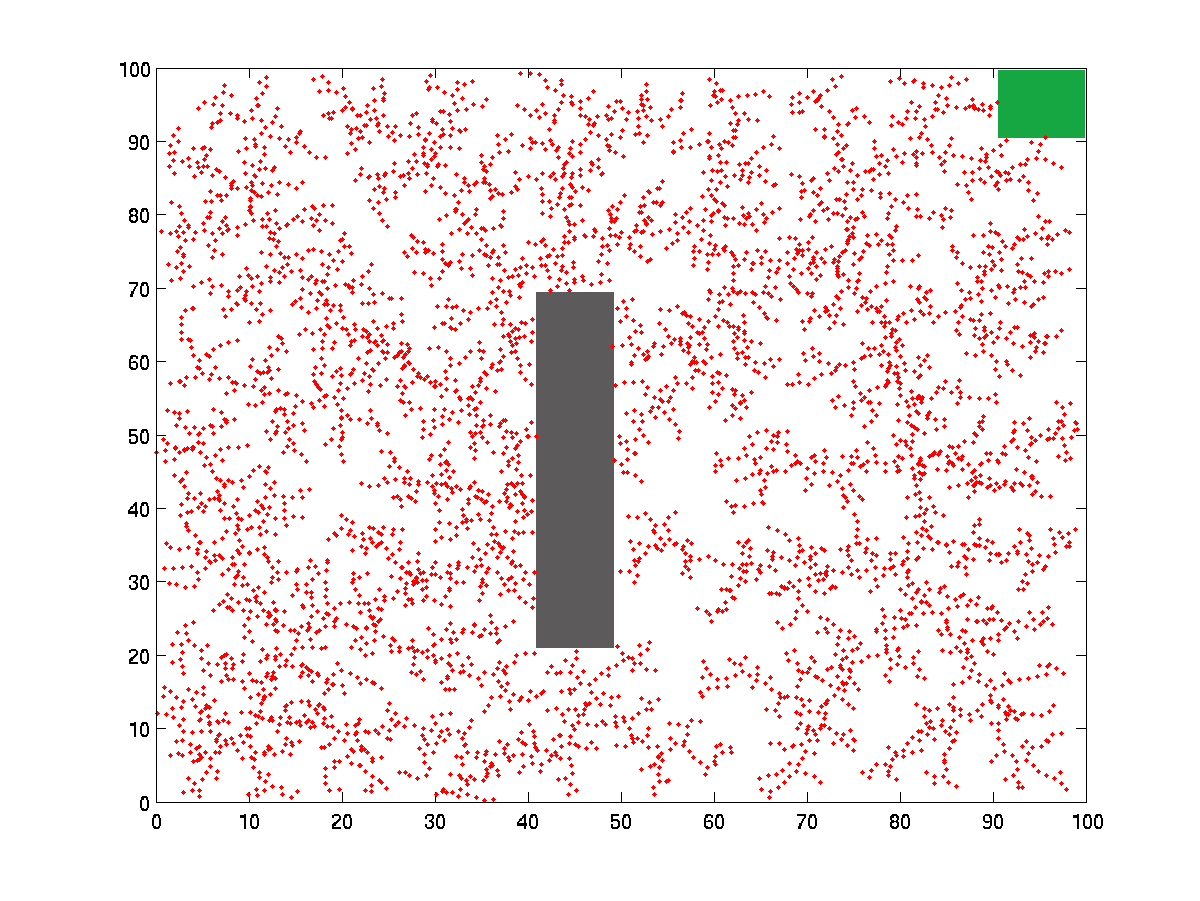
\includegraphics[width=0.45\linewidth]{i0_rrt.png}}%
    \qquad
    \subfigure[An instance of the approximated value function $V$]{\label{fig:vfunc}%
      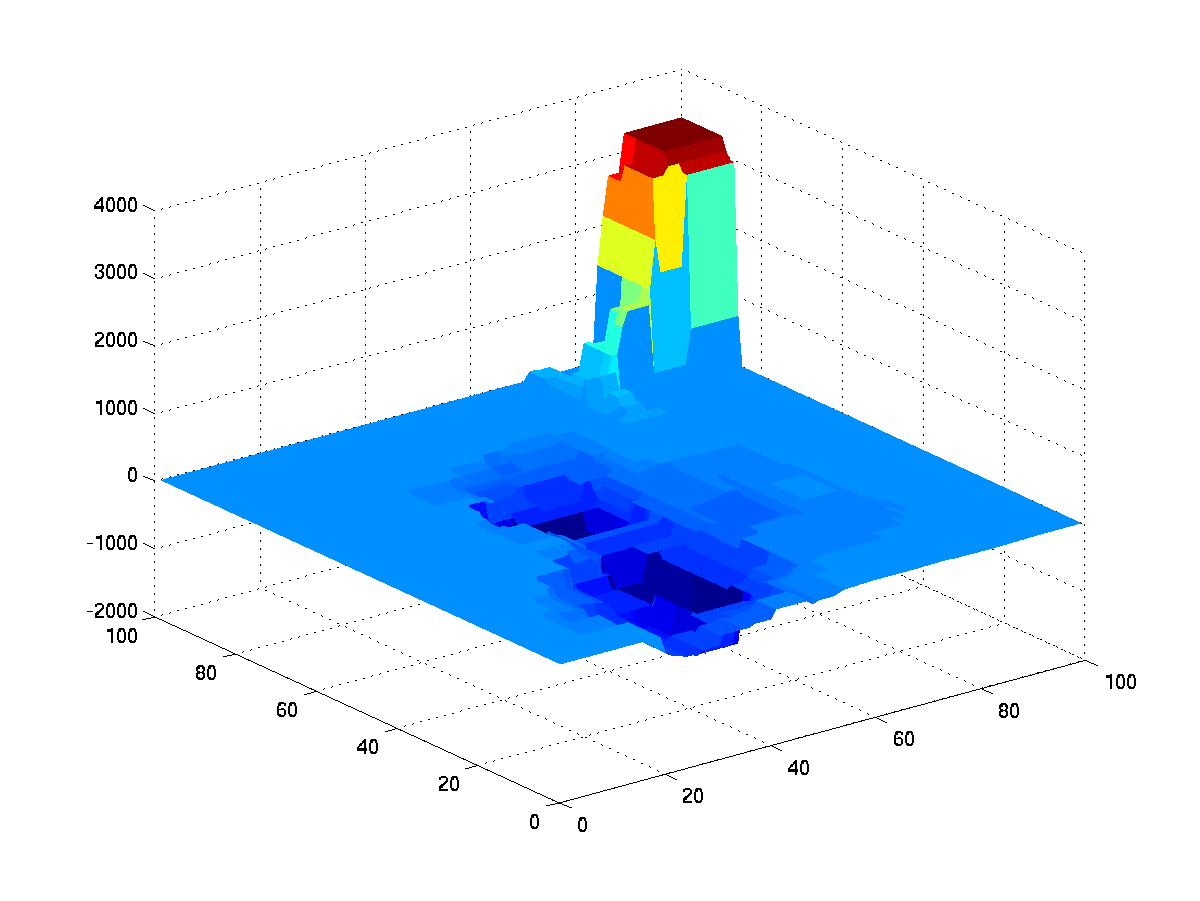
\includegraphics[width=0.45\linewidth]{vfunc.png}}
  }
\end{figure}
\begin{figure}[htbp]
\floatconts
  {fig:subfigex}
  {\caption{The trajectory corresponding to the leaf with largest value is shown in blue. The optimal trajectory is marked green. The policy on the right is clearly more optimal.}}
  {%
    \subfigure[Trajectory produced after a single iteration with 15000 samples]{\label{fig:rrtiter1}%
      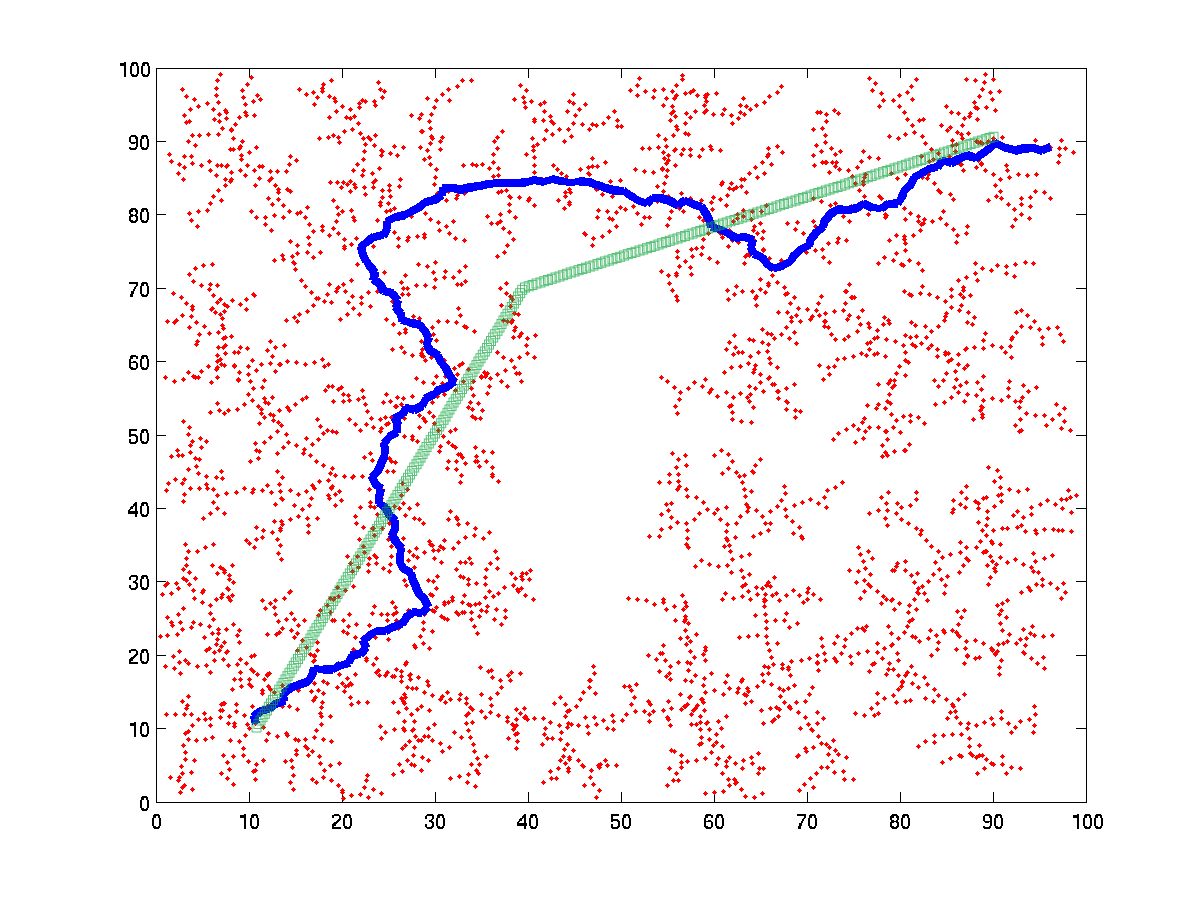
\includegraphics[width=0.45\linewidth]{bigrep.png}}%
    \qquad
    \subfigure[Trajectory produced after a 5 iterations of RRTPI with 3000 samples each ]{\label{fig:rrtiter5}%
      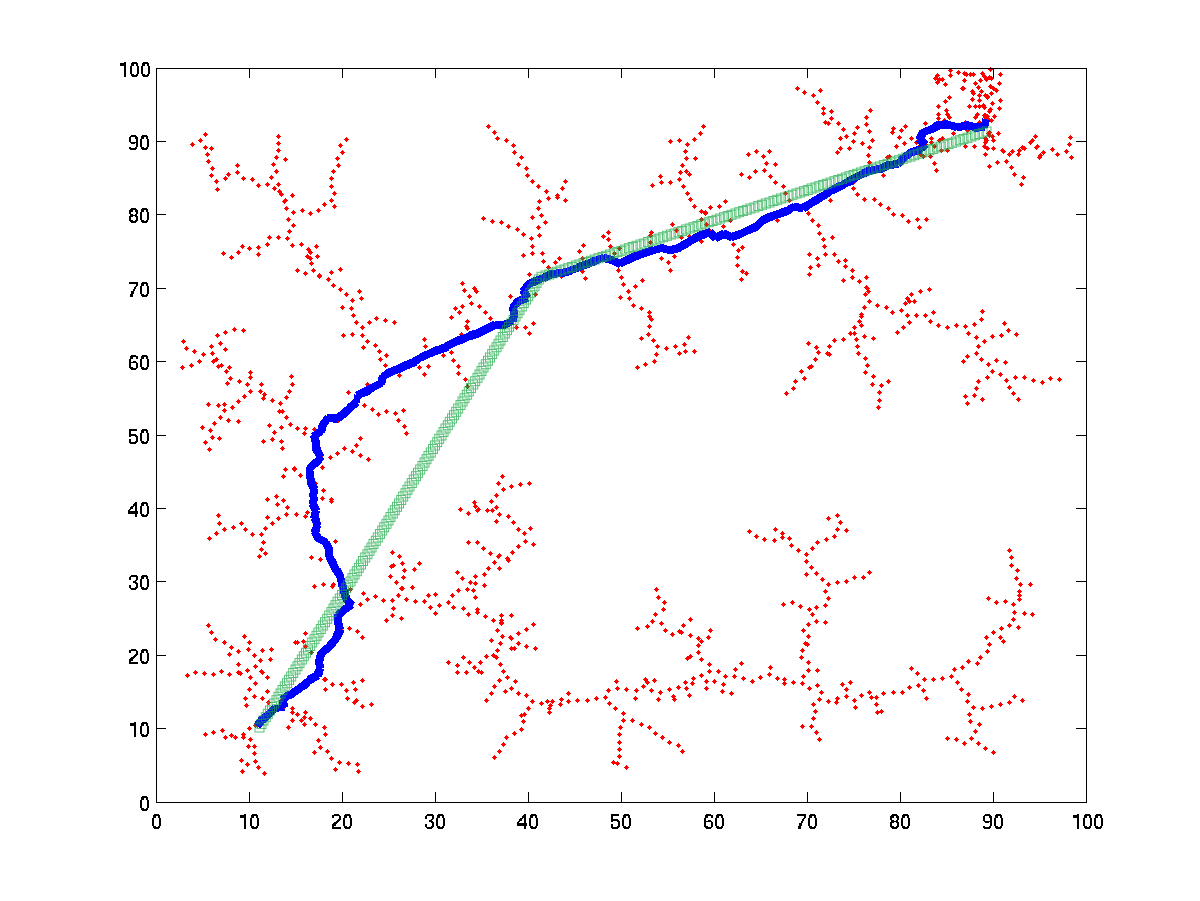
\includegraphics[width=0.45\linewidth]{smallrep.png}}
  }
\end{figure}

\section{Conclusion and Future Work}
In this paper we have presented a policy iteration method RRTPI that works on continuous state and action space MDPs. The RRTPI algorithm explicitly gives a method, based on RRTs, to generate samples from the domain, instead of assuming their availability. These trajectories have good exploration properties and their sample efficiency is empirically tested on a puddle world domain. A future direction of work would be to prove that the trajectories generated are fast-mixing, using results from \citep{karaman} on connections between random geometric graphs and RRTs. This result seems to be a key assumption in proving bounds on the sample complexity of the algorithm as hinted in \citep{antosml}.  

\bibliography{rrtpi}

\end{document}
